\documentclass[a4paper]{book}
\usepackage{a4wide}
\usepackage{makeidx}
\usepackage{graphicx}
\usepackage{multicol}
\usepackage{float}
\usepackage{listings}
\usepackage{color}
\usepackage{textcomp}
\usepackage{alltt}
\usepackage{times}
\usepackage{ifpdf}
\ifpdf
\usepackage[pdftex,
            pagebackref=true,
            colorlinks=true,
            linkcolor=blue,
            unicode
           ]{hyperref}
\else
\usepackage[ps2pdf,
            pagebackref=true,
            colorlinks=true,
            linkcolor=blue,
            unicode
           ]{hyperref}
\usepackage{pspicture}
\fi
\usepackage[utf8]{inputenc}
\usepackage{doxygen}
\lstset{language=C++,inputencoding=utf8,basicstyle=\footnotesize,breaklines=true,breakatwhitespace=true,tabsize=8,numbers=left }
\makeindex
\setcounter{tocdepth}{3}
\renewcommand{\footrulewidth}{0.4pt}
\begin{document}
\hypersetup{pageanchor=false}
\begin{titlepage}
\vspace*{7cm}
\begin{center}
{\Large Reference Manual}\\
\vspace*{1cm}
{\large Generated by Doxygen 1.7.1}\\
\vspace*{0.5cm}
{\small Sun Mar 11 2012 23:40:24}\\
\end{center}
\end{titlepage}
\clearemptydoublepage
\pagenumbering{roman}
\tableofcontents
\clearemptydoublepage
\pagenumbering{arabic}
\hypersetup{pageanchor=true}
\chapter{Class Index}
\section{Class Hierarchy}
This inheritance list is sorted roughly, but not completely, alphabetically:\begin{DoxyCompactList}
\item \contentsline{section}{BooleanExpression}{\pageref{classBooleanExpression}}{}
\item \contentsline{section}{IsAbleToPlay}{\pageref{interfaceIsAbleToPlay}}{}
\begin{DoxyCompactList}
\item \contentsline{section}{DumbComputerAI}{\pageref{classDumbComputerAI}}{}
\item \contentsline{section}{Human}{\pageref{classHuman}}{}
\end{DoxyCompactList}
\item \contentsline{section}{NimGame}{\pageref{classNimGame}}{}
\item \contentsline{section}{Readable}{\pageref{interfaceReadable}}{}
\begin{DoxyCompactList}
\item \contentsline{section}{Rebus}{\pageref{classRebus}}{}
\end{DoxyCompactList}
\item \contentsline{section}{VectorUtil}{\pageref{classVectorUtil}}{}
\item \contentsline{section}{XOBoard}{\pageref{classXOBoard}}{}
\item \contentsline{section}{XOGame}{\pageref{classXOGame}}{}
\end{DoxyCompactList}

\chapter{Class Index}
\section{Class List}
Here are the classes, structs, unions and interfaces with brief descriptions:\begin{DoxyCompactList}
\item\contentsline{section}{\hyperlink{classBooleanExpression}{BooleanExpression} }{\pageref{classBooleanExpression}}{}
\item\contentsline{section}{\hyperlink{classMaze}{Maze} }{\pageref{classMaze}}{}
\item\contentsline{section}{\hyperlink{classNimGameConf}{NimGameConf} }{\pageref{classNimGameConf}}{}
\item\contentsline{section}{\hyperlink{classRebus}{Rebus} }{\pageref{classRebus}}{}
\item\contentsline{section}{\hyperlink{classSudokuBoard}{SudokuBoard} }{\pageref{classSudokuBoard}}{}
\item\contentsline{section}{\hyperlink{classXOBoard}{XOBoard} }{\pageref{classXOBoard}}{}
\item\contentsline{section}{\hyperlink{classXOGame}{XOGame} }{\pageref{classXOGame}}{}
\end{DoxyCompactList}

\chapter{Class Documentation}
\hypertarget{classBooleanExpression}{
\section{BooleanExpression Class Reference}
\label{classBooleanExpression}\index{BooleanExpression@{BooleanExpression}}
}
\subsection*{Public Member Functions}
\begin{DoxyCompactItemize}
\item 
\hypertarget{classBooleanExpression_add76e02bf45058445aaf70fd6400108c}{
boolean {\bfseries isValid} ()}
\label{classBooleanExpression_add76e02bf45058445aaf70fd6400108c}

\item 
\hypertarget{classBooleanExpression_ae02cb61914b378cdd28cd858d9e8a4a0}{
Lexem\mbox{[}$\,$\mbox{]} {\bfseries getLexems} ()}
\label{classBooleanExpression_ae02cb61914b378cdd28cd858d9e8a4a0}

\end{DoxyCompactItemize}
\subsection*{Package Functions}
\begin{DoxyCompactItemize}
\item 
\hypertarget{classBooleanExpression_a0ac4c6f0eb4d1e9b96bd837aa31de159}{
{\bfseries BooleanExpression} (String stringRepresentation)}
\label{classBooleanExpression_a0ac4c6f0eb4d1e9b96bd837aa31de159}

\end{DoxyCompactItemize}


The documentation for this class was generated from the following file:\begin{DoxyCompactItemize}
\item 
/home/marcvs/Desktop/working/pa-\/materiale/pa/codeBase/Java/src/BooleanExpression.java\end{DoxyCompactItemize}

\hypertarget{interfaceReadable}{
\section{Readable Interface Reference}
\label{interfaceReadable}\index{Readable@{Readable}}
}
Inheritance diagram for Readable:\begin{figure}[H]
\begin{center}
\leavevmode
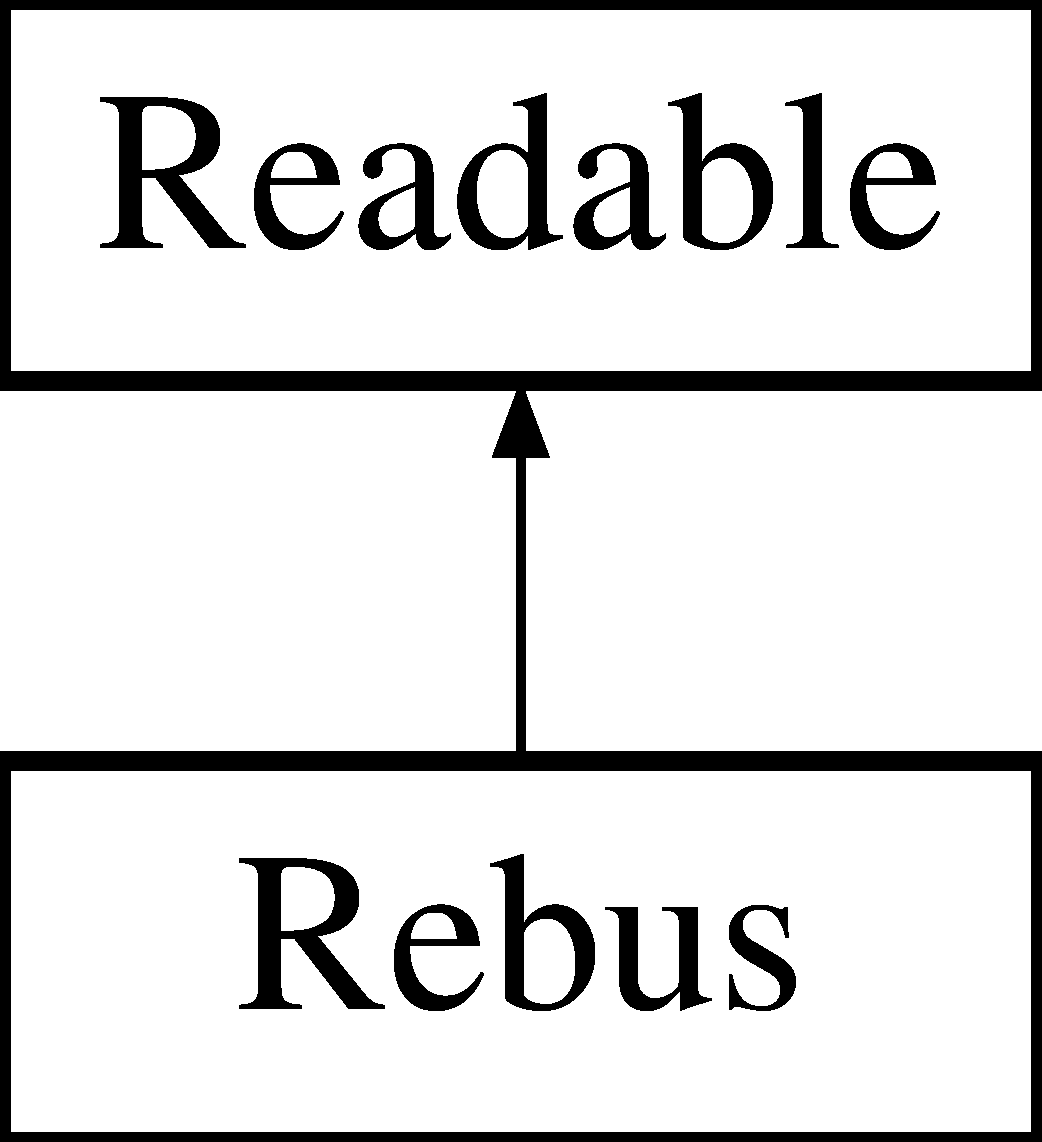
\includegraphics[height=2.000000cm]{interfaceReadable}
\end{center}
\end{figure}
\subsection*{Public Member Functions}
\begin{DoxyCompactItemize}
\item 
\hypertarget{interfaceReadable_a4ff1529890f69b2ad321bc06e497ed16}{
void {\bfseries read} (Scanner scanner)}
\label{interfaceReadable_a4ff1529890f69b2ad321bc06e497ed16}

\end{DoxyCompactItemize}


The documentation for this interface was generated from the following file:\begin{DoxyCompactItemize}
\item 
/home/marcvs/Desktop/working/pa-\/materiale/pa/codeBase/Java/src/Readable.java\end{DoxyCompactItemize}

\hypertarget{classRebus}{
\section{Rebus Class Reference}
\label{classRebus}\index{Rebus@{Rebus}}
}
Inheritance diagram for Rebus:\begin{figure}[H]
\begin{center}
\leavevmode
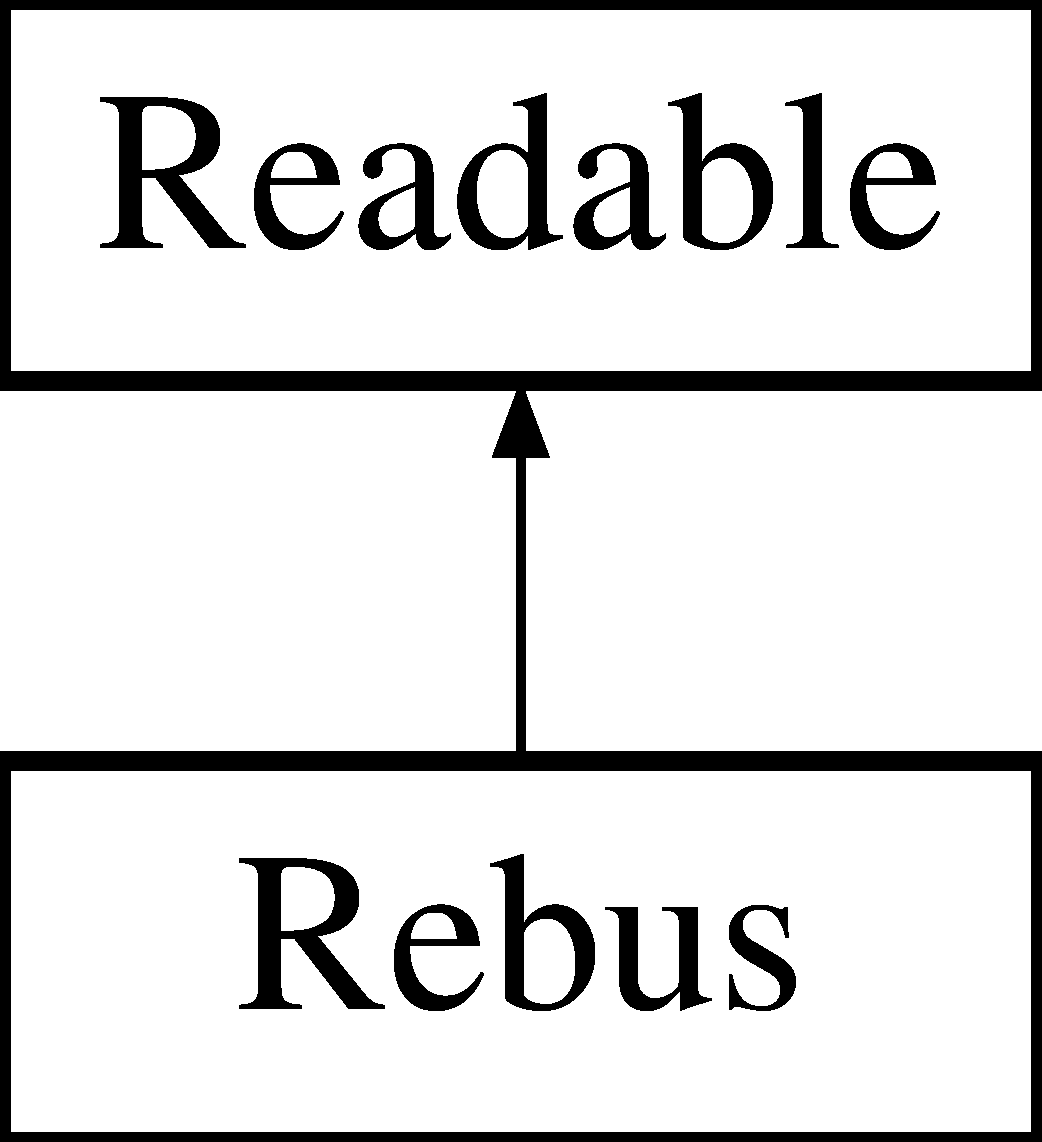
\includegraphics[height=2.000000cm]{classRebus}
\end{center}
\end{figure}
\subsection*{Public Member Functions}
\begin{DoxyCompactItemize}
\item 
\hypertarget{classRebus_a2495b8ab66b8b5fc73be661e6ccb85d3}{
char {\bfseries get} (int row, int column)}
\label{classRebus_a2495b8ab66b8b5fc73be661e6ccb85d3}

\item 
\hypertarget{classRebus_a33c68ead613e1cad7e1e274451f769c0}{
void {\bfseries put} (int row, int column, char c)}
\label{classRebus_a33c68ead613e1cad7e1e274451f769c0}

\item 
\hypertarget{classRebus_ab1ffa625317a5f6f05c75ec072a4bf53}{
void {\bfseries read} (Scanner scanner)}
\label{classRebus_ab1ffa625317a5f6f05c75ec072a4bf53}

\item 
\hypertarget{classRebus_ad208ddcbae9a498c5e8ef2beec2a3306}{
String {\bfseries toString} ()}
\label{classRebus_ad208ddcbae9a498c5e8ef2beec2a3306}

\end{DoxyCompactItemize}
\subsection*{Public Attributes}
\begin{DoxyCompactItemize}
\item 
\hypertarget{classRebus_a0d21b9515af691a04c515a3c163bd683}{
int {\bfseries rows}}
\label{classRebus_a0d21b9515af691a04c515a3c163bd683}

\item 
\hypertarget{classRebus_a71ec10584853e625028ea0c7c4932256}{
int {\bfseries columns}}
\label{classRebus_a71ec10584853e625028ea0c7c4932256}

\end{DoxyCompactItemize}
\subsection*{Package Functions}
\begin{DoxyCompactItemize}
\item 
\hypertarget{classRebus_ae7febf865939cb84fc08a087d12ee465}{
void {\bfseries putString} (int row, int column, String s)}
\label{classRebus_ae7febf865939cb84fc08a087d12ee465}

\item 
\hypertarget{classRebus_a7f568be5d10645247a9c3b9c3aefd31b}{
void {\bfseries eraseString} (int row, int column)}
\label{classRebus_a7f568be5d10645247a9c3b9c3aefd31b}

\item 
\hypertarget{classRebus_a51b184a4ff31ffb8d696daf86b6027f9}{
void {\bfseries erase} (int row, int column)}
\label{classRebus_a51b184a4ff31ffb8d696daf86b6027f9}

\item 
\hypertarget{classRebus_ad429f688c0bd500988843f21426bca97}{
boolean {\bfseries is\_\-empty} (int row, int column)}
\label{classRebus_ad429f688c0bd500988843f21426bca97}

\item 
\hypertarget{classRebus_a75a4903e5f1d6ecb72c3689fda4422f3}{
boolean {\bfseries is\_\-done} ()}
\label{classRebus_a75a4903e5f1d6ecb72c3689fda4422f3}

\end{DoxyCompactItemize}
\subsection*{Package Attributes}
\begin{DoxyCompactItemize}
\item 
\hypertarget{classRebus_aa874c93e563860b32ee8d70bd15b66c7}{
char\mbox{[}$\,$\mbox{]}\mbox{[}$\,$\mbox{]} {\bfseries m}}
\label{classRebus_aa874c93e563860b32ee8d70bd15b66c7}

\item 
\hypertarget{classRebus_a3279788d9a6d47b8c7bc6857582d298c}{
char\mbox{[}$\,$\mbox{]}\mbox{[}$\,$\mbox{]} {\bfseries ref}}
\label{classRebus_a3279788d9a6d47b8c7bc6857582d298c}

\end{DoxyCompactItemize}


The documentation for this class was generated from the following file:\begin{DoxyCompactItemize}
\item 
/home/marcvs/Desktop/working/pa-\/materiale/pa/codeBase/Java/src/Rebus.java\end{DoxyCompactItemize}

\hypertarget{classVectorUtil}{
\section{VectorUtil Class Reference}
\label{classVectorUtil}\index{VectorUtil@{VectorUtil}}
}
\subsection*{Static Public Member Functions}
\begin{DoxyCompactItemize}
\item 
\hypertarget{classVectorUtil_aff4c2878342ce74cd1dbed299fa16678}{
static$<$ T $>$ T\mbox{[}$\,$\mbox{]} {\bfseries readArrayOfReadables} (T\mbox{[}$\,$\mbox{]} vectorHint, Class classType)}
\label{classVectorUtil_aff4c2878342ce74cd1dbed299fa16678}

\item 
\hypertarget{classVectorUtil_a872045ae05e75378562d354bf14df5dd}{
static int\mbox{[}$\,$\mbox{]} {\bfseries readArrayOfIntegers} ()}
\label{classVectorUtil_a872045ae05e75378562d354bf14df5dd}

\end{DoxyCompactItemize}


The documentation for this class was generated from the following file:\begin{DoxyCompactItemize}
\item 
/home/marcvs/Desktop/working/pa-\/materiale/pa/codeBase/Java/src/VectorUtil.java\end{DoxyCompactItemize}

\printindex
\end{document}
